\documentclass[11pt]{article}
\usepackage[top=3cm, bottom=2.5cm, left=3cm, right=3cm]{geometry}
\usepackage{minted}
\usepackage{pgf}
\usepackage{tikz}
\usetikzlibrary{arrows,positioning,automata}
\usepackage{lmodern}
\usepackage{diagbox}
\usepackage[hidelinks, colorlinks=false]{hyperref}

\begin{document}
\title{RAPPORT IN406 : Evaluation d'expressions booléennes}
\author{Mohand Arezki ACHERIR 21921002 -- Clémence DUMOULIN 21903986}
\date{25 mai 2021}
\maketitle

\renewcommand*\contentsname{Sommaire}
\tableofcontents

\newpage
\section{Fonctionnement du programme}
\subsection{Organisation des fichiers}
L'implémentation de ce projet est en C, décomposée en deux fichiers. L'un correspondant à l'évaluation d'expression booléenne sans priorité entre les opérateurs \textbf{eval.c}, et l'autre à l'évaluation d'expression booléenne avec une priorité entre les opérateurs \textbf{evalprio.c}.

\subsection{Matériel de compilation}
\noindent Pour la compilation on utilise un \textbf{Makefile}, il suffit d'écrire la commande \textbf{make} ou \textbf{make test} pour compiler \textbf{eval.c} et lancer 5 exemples pertinents sur l'évaluation d'une expression booléenne. Pareillement, écrire la commande \textbf{make priorite} permet de compiler \textbf{evalprio.c} et lancer 6 exemples montrant les différences d'évaluation liées à la priorité des opérateurs. Ces expressions sont celles respectivement indiquées dans la cible \textbf{test} et dans la cible \textbf{priorite}. On peut les changer dans le Makefile, ou écrire \textbf{./eval "expression booléenne"} en ligne de commande. De plus, écrire \textbf{make debug} ou \textbf{make debugp} permet de vérifier à l'aide de Valgrind si la mémoire a bien été utilisée (allocation et libération de mémoire) dans chacun des cas énoncés ci-dessus. Enfin, la cible \textbf{clean} permet d'effacer les exécutables et de lister le contenu du répertoire courant.
\bigskip

\section{Raisonnement et description du programme}
Cette partie est divisée en quatre sous parties. Une pour la première question, une autre pour les questions deux et trois, la troisième pour les questions quatre et cinq, et la dernière pour la partie facultative.

\subsection{Transformation d'une chaine de caractère en liste de tokens}
On souhaite ici, lire une expression en argument, vérifier s'il s'agit bien d'une expression écrite avec l'alphabet du langage pour ensuite l'affecter à une liste chainée de token. On ne veut pas créer une liste de tokens si le mot est composé d'autres lettres que celles du langage. Par exemple, le mot \textbf{1+a} n'est pas transformé en liste de token puisque la lettre a n'appartient pas à notre alphabet. On supprime également les espaces s'il y en a pour ne pas stocker inutilement un espace dans un token.
De plus, on considère les mots en C, composés de plusieurs caractère, comme des lettres. Par exemple, NON est ajouté dans la liste, seulement si on lit un N, puis un O et un autre N, sinon NON n'est pas considéré comme une lettre de l'alphabet.
Ainsi, la fonction en C :
\begin{minted}{C}
liste_token creer_liste(char *string);
\end{minted}
permet de vérifier l'appartenance de chaque lettre à notre alphabet et de construire la liste de tokens comme liste chainée avec les fonctions
\begin{minted}{C}
liste_token creer_token(int type, char *op, char par, int value);
liste_token ajouter_fin_liste(liste_token current, liste_token add);
\end{minted}

\newpage
\subsection{Reconnaissance par automate}
On crée l'automate à pile $A = \{\Sigma,Q,q0,\Gamma,\delta,F,T\}$, tel que :

\noindent $\Sigma = \{0,1,NON,(,),.,+,=>,<=>\}$

\noindent $Q = \{q0,q1\}$

\noindent $\Gamma = \{X\}$

\noindent $F = \{q1\}$

\noindent $T = \left\{
    \begin{array}{c c c c c}
        (q0, & \delta, & (, & \delta X, & q0), \\
        (q0, & X, & (, & XX, & q0), \\
        (q0, & \delta, & NON, & \delta, & q0), \\
        (q0, & X, & NON, & X, & q0), \\
        (q0, & \delta, & 0, & \delta, & q1), \\
        (q0, & X, & 0, & X, & q1), \\
        (q0, & \delta, & 1, & \delta, & q1), \\
        (q0, & X, & 1, & X, & q1), \\
        (q1, & X, & ), & \epsilon, & q1), \\
        (q1, & \delta, & +, & \delta, & q0), \\
        (q1, & X, & +, & X, & q0), \\
        (q1, & \delta, & ., & \delta, & q0), \\
        (q1, & X, & ., & X, & q0), \\
        (q1, & \delta, & \Rightarrow, & \delta, & q0), \\
        (q1, & X, & \Rightarrow, & X, & q0), \\
        (q1, & \delta, & \Leftrightarrow, & \delta, & q0), \\
        (q1, & X, & \Leftrightarrow, & X, & q0), \\
    \end{array}
\right\}$

\bigskip
\bigskip
\noindent Ce qui nous donne, graphiquement :

\begin{center}
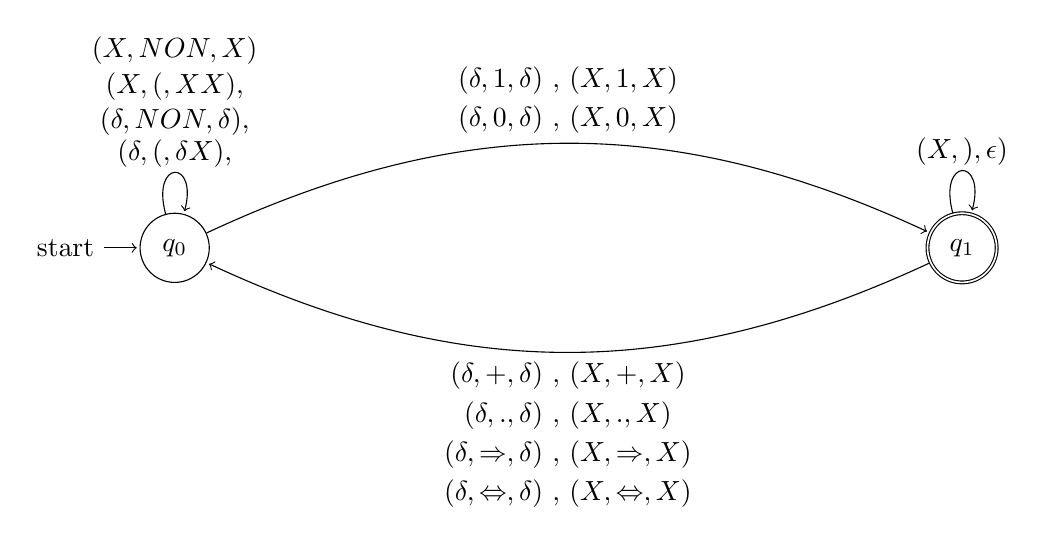
\begin{tikzpicture}[shorten >=1pt,node distance=10cm,on grid]
    \node[state,initial]  (q_0)        {$q_0$};
    \node[state,accepting]      (q_1) [right=of q_0] {$q_1$};
    \path[->] (q_0) edge [loop above] 
                            node[above=-0.05cm] {($\delta,(,\delta X$),} 
                            node[above = 0.80cm]{($X,(,XX$),}
                            node[above = 0.35cm]{($\delta,NON,\delta$),}
                            node[above = 1.25cm]{($X,NON,X$)} ()
            edge [bend left=25] node [above] {($\delta,0,\delta$) , ($X,0,X$)}
                                node [above = 0.5cm] {($\delta,1,\delta$) , ($X,1,X$)} (q_1)
      (q_1) edge [bend left=25] node [below] {($\delta,+,\delta$) , ($X,+,X$)}
                                node [below = 0.5cm] {($\delta,.,\delta$) , ($X,.,X$)}
                                node [below = 1cm] {($\delta,\Rightarrow,\delta$) , ($X,\Rightarrow,X$)}
                                node [below = 1.5cm] {($\delta,\Leftrightarrow,\delta$) , ($X,\Leftrightarrow,X$)} (q_0)
      (q_1) edge [loop above]  node[above=-0.05cm] {($X,),\epsilon$)} ();
\end{tikzpicture}
\end{center}

\noindent On fait une reconnaissance par pile vide et état final.

\noindent La pile de l'automate permet de vérifier la bonne position, et le bon nombre de parenthèses (ouvrantes et fermantes). L'état final permet de ne pas reconnaître une expression ne finissant ni par une constante, ni par une parenthèse fermante.

\noindent Pour construire cet automate, on a utilisé le tableau ci-dessous, qui permet de savoir quelle lettre peut directement se trouver à la suite d'une autre.

\begin{center}
\begin{tabular}{|c|c c c c c c c c c c|}
    \hline
    \diagbox{$courant$}{$suivant$} & ( & ) & 0 & 1 & NON & + & . & $\Rightarrow$ & $\Leftrightarrow$ & Fin\\
    \hline
    ( & X & & X & X & X & & & & & \\
    ) & & X & & & & X & X & X & X & X \\
    0 & & X & & & & X & X & X & X & X \\
    1 & & X & & & & X & X & X & X & X \\
    NON & X & & X & X & X & & & & & \\
    + & X & & X & X & X & & & & & \\
    . & X & & X & X & X & & & & & \\
    $\Rightarrow$ & X & & X & X & X & & & & &\\
    $\Leftrightarrow$ & X & & X & X & X & & & & &\\
    Initial & X & & X & X & X & & & & &\\
    \hline
\end{tabular}
\end{center}
On remarque deux statuts différents, correspondant aux deux états de notre automate. Les boucles sur un état se justifient par un élément qui peut se suivre lui-même (la diagonale du tableau).

\noindent L'implémentation en C se fait avec la fonction, ci-dessous, qui renvoie 0 quand l'expression n'est pas reconnu par l'automate et 1 sinon.
\begin{minted}{C}
int est_valide(liste_token lt);
\end{minted}

\subsection{Arbre et évaluation de l'expression}
Dans cette partie, l'objectif est de rechercher l'opérateur de priorité la plus faible. Cependant, on ne considère pas la priorité entre les opérateurs, ainsi l'opérateur le moins prioritaire devient le dernier dans l'ordre de lecture en dehors des parenthèses. On considère tout de même que sans parenthèse l'opérateur unaire NON est prioritaire. Par exemple, dans l'expression $1\Rightarrow NON 1$, $NON 1$ sera effectué avant l'implication. L'opérateur le moins prioritaire sera effectué en dernier. Cette recherche se fait dans la fonction :
\begin{minted}{C}
liste_token chrch_opp(liste_token lt, int nb)
\end{minted}
\noindent Une fois cet opérateur trouvé, on l'affecte en racine de l'arbre et on découpe la liste chaînée en deux, la partie précédant l'opérateur et la partie suivant l'opérateur. Le fils gauche de la racine sera la partie précédant l'opérateur, et le fils droit, la partie le suivant. Ceci est permis grâce aux fonctions :
\begin{minted}{C}
liste_token get_prev(liste_token lt, liste_token t, int nb);
liste_token get_next(liste_token lt, liste_token t, int nb);
\end{minted}
On répète ces étapes récursivement jusqu'à finir la construction de l'arbre.

\noindent Nous avons choisi d'afficher l'arbre en parcours postfixe puisque combiné à l'expression en argument, qui correspond à un parcours infixe, on peut vérifier que l'arbre est correctement construit.
\bigskip

\noindent Après avoir construit l'arbre, on évalue l'expression remontant l'arbre. Lorsqu'on atteint une feuille, on stocke sa valeur dans une variable et on remonte au père pour effectuer l'opération correspondante à l'opérateur stocké dans ce noeud. L'évaluation se fait grâce à la fonction : 
\begin{minted}{C}
int arbre_to_int(arbre_token at);
\end{minted}
\newpage

\subsection{Avec priorité des opérateurs}
Dans cette partie, il suffit seulement d'intégrer une fonction qui indique la priorité suivie par les opérateurs. On définit les opérateurs du plus prioritaire au moins prioritaire : 
\begin{itemize}
    \item $()$ 
    \item $NON$ 
    \item $.$ 
    \item $+$ 
    \item $\Rightarrow$ 
    \item $\Leftrightarrow$
\end{itemize}

\noindent On implémente cette priorité par la fonction :
\begin{minted}{C}
int is_weaker(liste_token curr, liste_token opp);
\end{minted}
Il faut également une petite modification dans la recherche de l'opérateur racine de l'arbre, lorsqu'on compare deux opérateurs entre eux, dans la fonction :
\begin{minted}{C}
liste_token chrch_opp(liste_token lt, int nb);
\end{minted}

\end{document}
